\section{量子フーリエ変換}
\label{sec:quantum-fourier-transform}

\subsection{定義}
\label{subsec:qft-definition}

量子コンピュータで離散フーリエ変換を行うサブルーチンを
\textbf{量子フーリエ変換}という\cite{shimada2020}．
$t$を正の整数とし，$t$量子ビットの計算基底状態の総数を
\begin{equation}
  M
  \coloneq
  2^t
  \label{eq:qft-dimension}
\end{equation}
とする．量子状態の振幅として用いる複素数の配列
$\{x_j\}_{j=0}^{M-1}$は，規格化条件
\begin{equation}
  \sum_{j=0}^{M-1}|x_j|^2
  =
  1
  \label{eq:qft-amplitude-normalization}
\end{equation}
を満たすものとする．この配列に対する離散フーリエ変換を
\begin{equation}
  y_k
  \coloneq
  \frac{1}{\sqrt{M}}
  \sum_{j=0}^{M-1}
  x_j
  \exp\left(
    \frac{2\pi\mathrm{i}kj}{M}
  \right),
  \qquad
  k=0,1,\ldots,M-1
  \label{eq:qft-output-amplitude}
\end{equation}
と定義する．ここで，$\mathrm{i}$は虚数単位である．

入力と出力を列ベクトル
\begin{equation}
  \bm{x}
  \coloneq
  \begin{bmatrix}
    x_0 & x_1 & \cdots & x_{M-1}
  \end{bmatrix}^{\mathsf{T}},
  \qquad
  \bm{y}
  \coloneq
  \begin{bmatrix}
    y_0 & y_1 & \cdots & y_{M-1}
  \end{bmatrix}^{\mathsf{T}}
  \label{eq:qft-vector-definitions}
\end{equation}
とする．また，$M\times M$行列$W$の行列要素を
\begin{equation}
  W_{kj}
  \coloneq
  \left[
    \exp\left(
      \frac{2\pi\mathrm{i}}{M}
    \right)
  \right]^{kj},
  \qquad
  j,k=0,1,\ldots,M-1
  \label{eq:qft-fourier-matrix-elements}
\end{equation}
と定義すれば，式\eqref{eq:qft-output-amplitude}は
\begin{equation}
  \bm{y}
  =
  \frac{1}{\sqrt{M}}W\bm{x}
  \label{eq:qft-matrix-form}
\end{equation}
と表される．

次に，$\bm{x}$と$\bm{y}$をそれぞれ振幅符号化した量子状態を
\begin{equation}
  \ket{x}
  \coloneq
  \sum_{j=0}^{M-1}x_j\ket{j},
  \qquad
  \ket{y}
  \coloneq
  \sum_{k=0}^{M-1}y_k\ket{k}
  \label{eq:qft-state-definitions}
\end{equation}
と定義する．量子フーリエ変換$F_M$は，これらの状態の間を
\begin{equation}
  F_M\ket{x}
  =
  \ket{y}
  \label{eq:qft-state-transformation}
\end{equation}
と変換するユニタリ演算子である．式\eqref{eq:qft-output-amplitude}と
式\eqref{eq:qft-state-definitions}より，出力状態は
\begin{align}
  \ket{y}
  &=
  \frac{1}{\sqrt{M}}
  \sum_{k=0}^{M-1}
  \sum_{j=0}^{M-1}
  x_j
  \exp\left(
    \frac{2\pi\mathrm{i}kj}{M}
  \right)
  \ket{k}
  \notag\\
  &=
  \sum_{j=0}^{M-1}
  x_j
  \left(
    \frac{1}{\sqrt{M}}
    \sum_{k=0}^{M-1}
    \exp\left(
      \frac{2\pi\mathrm{i}kj}{M}
    \right)
    \ket{k}
  \right)
  \label{eq:qft-output-state-expansion}
\end{align}
と変形できる．第1式から第2式への変形では，有限和の順序を入れ替え，
入力振幅$x_j$ごとに項をまとめている．一方，入力状態は
$\ket{x}=\sum_{j=0}^{M-1}x_j\ket{j}$であるため，線形性より，
量子フーリエ変換は各計算基底状態に対して
\begin{equation}
  F_M\ket{j}
  =
  \frac{1}{\sqrt{M}}
  \sum_{k=0}^{M-1}
  \exp\left(
    \frac{2\pi\mathrm{i}kj}{M}
  \right)
  \ket{k},
  \qquad
  j=0,1,\ldots,M-1
  \label{eq:qft-definition}
\end{equation}
と作用する．

式\eqref{eq:qft-definition}を量子ビットごとの積へ分解するため，
入力側の整数$j$と出力側の整数$k$をそれぞれ
\begin{align}
  j
  &=
  j_1 2^{t-1}+j_2 2^{t-2}+\cdots+j_t,
  \notag\\
  k
  &=
  k_1 2^{t-1}+k_2 2^{t-2}+\cdots+k_t,
  \qquad
  j_r,k_r\in\{0,1\}
  \label{eq:qft-binary-integer-definitions}
\end{align}
と2進展開する．このとき
\begin{equation}
  \ket{k}
  =
  \ket{k_1k_2\cdots k_t}
  =
  \ket{k_1}\otimes\ket{k_2}\otimes\cdots\otimes\ket{k_t}
  \label{eq:qft-computational-basis-product}
\end{equation}
である．また，2進小数を
\begin{equation}
  0.j_rj_{r+1}\cdots j_t
  \coloneq
  \frac{j_r}{2}
  +\frac{j_{r+1}}{2^2}
  +\cdots
  +\frac{j_t}{2^{t-r+1}}
  \label{eq:qft-binary-fraction-definition}
\end{equation}
と定義する．

出力側の整数$k$を式\eqref{eq:qft-binary-integer-definitions}のように分解して
式\eqref{eq:qft-definition}へ代入すると，
\begin{align}
  F_M\ket{j}
  &=
  \frac{1}{2^{t/2}}
  \sum_{k_1=0}^{1}\cdots\sum_{k_t=0}^{1}
  \exp\left[
    2\pi\mathrm{i}j
    \left(
      k_1 2^{-1}+k_2 2^{-2}+\cdots+k_t 2^{-t}
    \right)
  \right]
  \ket{k_1k_2\cdots k_t}
  \notag\\
  &=
  \frac{1}{2^{t/2}}
  \bigotimes_{r=1}^{t}
  \left(
    \sum_{k_r=0}^{1}
    e^{2\pi\mathrm{i}jk_r/2^r}\ket{k_r}
  \right)
  \notag\\
  &=
  \frac{1}{2^{t/2}}
  \bigotimes_{r=1}^{t}
  \left(
    \ket{0}
    +e^{2\pi\mathrm{i}j/2^r}\ket{1}
  \right)
  \notag\\
  &=
  \frac{1}{2^{t/2}}
  \bigotimes_{r=1}^{t}
  \left(
    \ket{0}
    +e^{2\pi\mathrm{i}(0.j_{t-r+1}\cdots j_t)}\ket{1}
  \right)
  \label{eq:qft-product-decomposition}
\end{align}
となる．第1式から第2式への変形では，指数関数の積
$e^{a+b}=e^a e^b$とテンソル積の分配則を用いた．また，最後の変形では，
$j/2^r$の整数部分が$e^{2\pi\mathrm{i}m}=1$（$m$は整数）を満たすため，
小数部分$0.j_{t-r+1}\cdots j_t$だけが位相に寄与することを用いた．

\subsection{量子回路による実装と逆変換}
\label{subsec:qft-circuit-construction}

式\eqref{eq:qft-product-decomposition}の積状態は，Hadamardゲートと
制御位相ゲートを組み合わせて生成できる．まず，$\ell\geq2$に対して位相ゲート
\begin{equation}
  R_\ell
  \coloneq
  \begin{bmatrix}
    1 & 0\\
    0 & e^{2\pi\mathrm{i}/2^\ell}
  \end{bmatrix}
  \label{eq:qft-phase-gate}
\end{equation}
を定義する．制御$R_\ell$ゲートは，制御量子ビットと標的量子ビットが
ともに$\ket{1}$である場合に限り，振幅へ位相$e^{2\pi\mathrm{i}/2^\ell}$を付加する．
計算基底$\ket{00},\ket{01},\ket{10},\ket{11}$の順に表せば，その行列は
\begin{equation}
  \operatorname{C}R_\ell
  =
  \operatorname{diag}
  \left(
    1,1,1,e^{2\pi\mathrm{i}/2^\ell}
  \right)
  \label{eq:qft-controlled-phase-gate}
\end{equation}
である．

入力を$\ket{j_1j_2\cdots j_t}$とする．第1量子ビットへHadamardゲートを
作用させると
\begin{equation}
  \ket{j_1}
  \xmapsto{H}
  \frac{1}{\sqrt{2}}
  \left(
    \ket{0}
    +e^{2\pi\mathrm{i}(0.j_1)}\ket{1}
  \right)
  \label{eq:qft-first-hadamard}
\end{equation}
となる．次に，第2量子ビットを制御部，第1量子ビットを標的部とする
制御$R_2$ゲートを作用させると，$j_2=1$の場合に位相$2\pi/2^2$が加わる．
さらに，第3量子ビットから第$t$量子ビットまでを制御部とする
制御$R_3,\ldots,R_t$ゲートを順に作用させることで，第1量子ビットは
\begin{equation}
  \frac{1}{\sqrt{2}}
  \left(
    \ket{0}
    +e^{2\pi\mathrm{i}(0.j_1j_2\cdots j_t)}\ket{1}
  \right)
  \label{eq:qft-first-output-qubit}
\end{equation}
となる．

同様に，第$r$量子ビットへHadamardゲートを作用させた後，
第$r+1,\ldots,t$量子ビットを制御部とする
制御$R_2,\ldots,R_{t-r+1}$ゲートを順に作用させる．この処理により，
第$r$量子ビットは
\begin{equation}
  \ket{j_r}
  \longmapsto
  \frac{1}{\sqrt{2}}
  \left(
    \ket{0}
    +e^{2\pi\mathrm{i}(0.j_rj_{r+1}\cdots j_t)}\ket{1}
  \right)
  \label{eq:qft-rth-output-qubit}
\end{equation}
へ変換される．したがって，すべての量子ビットに対する処理を終えた状態は
\begin{equation}
  \frac{1}{2^{t/2}}
  \bigotimes_{r=1}^{t}
  \left(
    \ket{0}
    +e^{2\pi\mathrm{i}(0.j_rj_{r+1}\cdots j_t)}\ket{1}
  \right)
  \label{eq:qft-circuit-output-before-swaps}
\end{equation}
である．式\eqref{eq:qft-circuit-output-before-swaps}は，
式\eqref{eq:qft-product-decomposition}と量子ビットの順序が逆になっている．
そこで，第1量子ビットと第$t$量子ビット，第2量子ビットと第$t-1$量子ビットというように
SWAPゲートを作用させ，量子ビットの順序を反転する．これにより，
式\eqref{eq:qft-definition}で定義した量子フーリエ変換$F_M$が完成する．

図\ref{fig:qft-circuit-four-qubit}に，$t=4$の場合の量子フーリエ変換回路を示す．
回路は左から右へ進み，黒丸は制御量子ビット，$R_\ell$と書かれた箱は
標的量子ビットへ作用する位相ゲートを表す．図の右端では，2組のSWAPゲートによって
第1量子ビットと第4量子ビット，第2量子ビットと第3量子ビットを交換している．
一般の$t$量子ビットの場合も，同じ三角形状の配置を$t$本の量子ビット線へ拡張する．

\begin{figure}[tbp]
  \centering
  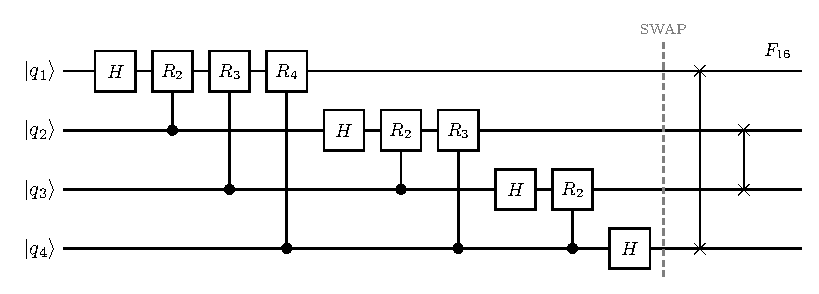
\includegraphics[width=0.92\textwidth]{figures/quantum-fourier-transform/qft-circuit.pdf}
  \caption{4量子ビット量子フーリエ変換の回路．$R_\ell$は式\eqref{eq:qft-phase-gate}で
  定義した位相ゲートであり，黒丸と$R_\ell$を結ぶ線は制御$R_\ell$ゲートを表す．
  右端の$\times$印はSWAPゲートを表す．}
  \label{fig:qft-circuit-four-qubit}
\end{figure}

量子フーリエ変換の逆変換は，随伴演算子$F_M^\dagger$であり，
計算基底に対して
\begin{equation}
  F_M^\dagger\ket{k}
  =
  \frac{1}{\sqrt{M}}
  \sum_{j=0}^{M-1}
  \exp\left(
    -\frac{2\pi\mathrm{i}kj}{M}
  \right)
  \ket{j}
  \label{eq:inverse-qft-definition}
\end{equation}
と作用する．逆量子フーリエ変換の回路は，量子フーリエ変換回路のゲートを
逆順に並べ，各位相ゲートを$R_\ell^\dagger$へ置き換えることで得られる．
量子位相推定では，補助量子ビットの相対位相に書き込まれた情報を
計算基底のビット列として読み出すために，この逆量子フーリエ変換を用いる．

\subsection{回路規模と読み出し}
\label{subsec:qft-circuit-size-and-readout}

厳密な$t$量子ビット量子フーリエ変換では，第$r$量子ビットに対して
1個のHadamardゲートと$t-r$個の制御位相ゲートを用いる．したがって，
SWAPゲートを除くゲート数は
\begin{equation}
  \sum_{r=1}^{t}
  \bigl(1+t-r\bigr)
  =
  \frac{t(t+1)}{2}
  \label{eq:qft-gate-count-without-swaps}
\end{equation}
である．内訳は，$t$個のHadamardゲートと$t(t-1)/2$個の制御位相ゲートである．
さらに量子ビットの順序を反転するには$\lfloor t/2\rfloor$個のSWAPゲートが必要であり，
各SWAPゲートを3個のCNOTゲートへ分解する場合には
$3\lfloor t/2\rfloor$個のCNOTゲートを用いる．したがって，厳密な量子フーリエ変換の
ゲート数は
\begin{equation}
  O(t^2)
  =
  O\bigl((\log M)^2\bigr)
  \label{eq:qft-gate-complexity}
\end{equation}
である\cite{shimada2020}．

一方，$M$点の離散フーリエ変換を古典コンピュータ上の高速フーリエ変換で
計算する場合の計算量は$O(M\log M)$である．ただし，この比較は，量子状態$\ket{x}$が
既に準備されており，出力を量子状態$\ket{y}$のまま後続の量子回路で利用する場合の
変換部分だけを比べたものである．古典データから$\ket{x}$を準備する計算量や，
量子状態から古典情報を読み出す計算量は含まれていない．

また，$\ell$が大きい位相ゲート$R_\ell$の回転角$2\pi/2^\ell$は小さい．
そこで，許容誤差に応じて小さな回転角を持つ制御位相ゲートを省略すれば，
近似量子フーリエ変換として回路を短くできる．必要な精度と回路深さの間には
トレードオフがあるため，後続処理で必要となる位相精度に応じて省略範囲を決める．

量子フーリエ変換の出力$\ket{y}$を計算基底で測定したとき，
整数$k$を得る確率は
\begin{equation}
  p_k
  =
  |y_k|^2
  \label{eq:qft-measurement-probability}
\end{equation}
であり，一度の測定から得られるのは一つのビット列だけである．
したがって，量子フーリエ変換を適用しただけでは，$M$個の複素フーリエ係数
$y_0,y_1,\ldots,y_{M-1}$をすべて古典的に得ることはできない．
すべての出力確率を推定するには回路の実行と測定を多数回繰り返す必要があり，
複素振幅の位相まで復元するにはさらに量子状態トモグラフィなどの処理が必要となる．
そのため，全フーリエ係数を列挙すること自体が目的であれば，量子フーリエ変換の
ゲート数だけを根拠として高速化を主張することはできない．

量子アルゴリズムでは，フーリエ変換後の状態を測定前に後続の量子回路へ入力し，
干渉によって必要な測定結果へ確率を集中させる．量子位相推定は，
この性質と逆量子フーリエ変換を用いて，固有位相に関する情報を選択的に読み出す．
